\documentclass[journal=jacsat,manuscript=article]{achemso}

\usepackage[version=3]{mhchem}
\usepackage{booktabs}
\usepackage{float}
\usepackage{amsmath}

\newcommand*\mycommand[1]{\texttt{\emph{#1}}}

\author{Cong Wen}
\author{Xiao Tan}
\author{Wen-Hao Li}
\author{Hong-Jin Chen}
\author{Jian-Tao Zai}
%\altaffiliation{Current address: Dormitary X13 104}
\affiliation[SJTU]
    {School of Chemistry and Chemical Engineering, Shanghai Jiao Tong University, Shanghai 200240, P. R. China}
\email{zaijiantao@sjtu.edu.cn}
\phone{+86-21-34202642}

\title{Spectrophotometric Determination of Iron Using Phenanthroline}

\abbreviations{SP,phen}
\keywords{Spectrophotometric,asd}

\begin{document}


% █████  ██████  ███████ ████████ ██████   █████   ██████ ████████
%██   ██ ██   ██ ██         ██    ██   ██ ██   ██ ██         ██
%███████ ██████  ███████    ██    ██████  ███████ ██         ██
%██   ██ ██   ██      ██    ██    ██   ██ ██   ██ ██         ██
%██   ██ ██████  ███████    ██    ██   ██ ██   ██  ██████    ██

\begin{abstract}

\textsf{Spectrophotometry} is an attractive alternative to titration method and gravimetric method when determining the concentration of metal ions, but there are many options in chromogenic agent, pH and chromogenic time, we choose phenanthroline as chromogenic agent and apply \textsf{orthogonal experimental design} to optimize the combination. We then used and compared \textsf{Job method} with \textsf{molar ratio method} in the determination of the composition of Tris(1,10-phenantholine) iron, we hold the opinion that molar ratio method is more general and more effective in this experiment. Under the optimized condition, we can plot a standard curve from measurement of ferric standard solutions of gradiently ascending consentration, with which we can reasonably predict the purity of our self-made iron(II) oxalate dihydrate; we get results very close to what is measured using titration method, while titration method behaves much worse in respect of meeting the requirements of green chemistry.

\end{abstract}

%██ ███    ██ ████████ ██████   ██████
%██ ████   ██    ██    ██   ██ ██    ██
%██ ██ ██  ██    ██    ██████  ██    ██
%██ ██  ██ ██    ██    ██   ██ ██    ██
%██ ██   ████    ██    ██   ██  ██████


\section{Introduction}
Iron is the most used metal in the world, and is broadly distributed in nature and human bodies, so we need a green, effective and efficient method to determine iron of ordinary, micro, trace quantity in samples such as minerals, blood plasma or serum\cite{Ramsay1957The,Wong1923COLORIMETRIC} and plants\cite{Reis1994Multicommutation, Suo-YiHuang2004DeterminationofIron}. As is widely accepted, titration method and gravimetry method behave very well when determining metal ions of ordinary quantity. However, they both fail to work if micro or trace analysis is required, futhermore, neither redox titration nor coordination titration is a preferred choice for the green determination of iron, meanwhile, gravimetry method is complicated and finicky to operate. spectrophotometry based on Beer-Lambert Law promise a larger potential as green and effecive methods to determine iron of either ordinary or trace quantity\cite{King1991Spectrophotometric,Carter1971Spectrophotometric,T1975Nitrosophenol}. Actually there are many options in chromogenic agent \cite{Yoe1944Colorimetric,Stookey1970Ferrozine,Er-KunShang20134}, and we choose phenanthroline as chromogenic agent and apply orthogonal experimental design to optimize the combination of wavelength($\lambda$), pH(amount of \ce{NaAc}), chromogenic time and amount of phenanthroline thereby improving accuracy of our following measurement. This method is undoubtedly the most direct approach to meet the requirements of green chemistry.\\
Phenanthroline(phen) is a heterocyclic organic compound. It is a white solid that is soluble in organic solvents. Phenanthroline is always used as a ligand in coordination chemistry, which can form strong complexes with iron ions. To use spectrophotometry properly, we apply this method to four experiments under the optimized condition:
\begin{enumerate}
    \item Determine the composition of the complex
    \begin{enumerate}
        \item Job method
        \item Molar ratio method
    \end{enumerate}
    \item Determine the concentration of iron ion
    \begin{enumerate}
        \item Plot the standard curve
        \item Determine the purity of \ce{FeC2O4}$\cdot$2\ce{H2O}
    \end{enumerate}
\end{enumerate}
In the first part, we we found in the complex the ratio of phen and iron is 3:1, meanwhile, we compared Job method and molar ratio method carefully and draw the conclusion that molar ratio method is much better because of higher degree of accuracy than Job method. In the second part, we first prepare standard ferric solutions of gradiently ascending concentration under optimum condition, then we plot the standard curve with measurement of each sample. Using the standard curve, we soon get the concentration of iron in our \ce{FeC2O4}$\cdot$2\ce{H2O} samples, therefore getting the purity; comparing with the experimental result of titration method, there is little difference.

%███████ ██   ██ ██████  ███████ ██████
%██       ██ ██  ██   ██ ██      ██   ██
%█████     ███   ██████  █████   ██████
%██       ██ ██  ██      ██      ██   ██
%███████ ██   ██ ██      ███████ ██   ██
%\mycommand{}
\section{Experimental}
\paragraph{Synthesis of \ce{FeC2O4}$\cdot$2\ce{H2O}}
\ce{(NH4)2Fe(SO4)2} (10.00g) was dissolved in 15mL deionized water, and the solution was acidized with 2mol/L \ce{H2SO4} (3mL); the beaker was heated until \ce{(NH4)2Fe(SO4)2} dissolved completely. Then 1mol/L \ce{H2C2O4} (60mL) was added into the beaker, and the solution was heated until it boiled, stirring continuously was necessary to prevent splashing. After standing precipitation for a while, the supernatant should be poured out. Then the precipitation was well washed by deionized water and collected by suction filtration. The product was washed by acetone twice and then dried and weighed for further use.
\paragraph{Orthogonal experiment}
 We studied four factors that have five levels each, and they are shown in Table~\ref{Tab.Fac} below.
\begin{table}[H]
  \caption{Factors}
  \label{Tab.Fac}
  \begin{tabular}{lcccc}
    \toprule
    Index & $\lambda /nm$ & $V_{\ce{phen}}/mL$ & $V_{\ce{NaAc}}/mL$ & T/min\\
    \midrule
    1     & 488           & 0.5                & 1                  & 4    \\
    2     & 498           & 1                  & 3                  & 6    \\
    3     & 508           & 2                  & 5                  & 8    \\
    4     & 518           & 3                  & 7                  & 10   \\
    5     & 528           & 4                  & 9                  & 12   \\
    \bottomrule
  \end{tabular}
\end{table}

We first prepared $0.15\%$ phen solution, 1mol/L \ce{NaAc} solution, $10\%$ hydroxylamine hydrochloride solution, $100\mu g\cdot cm^{-3}$  and $20\mu g\cdot cm^{-3}$ ferric standard solution. The \ce{NaAc} solution could be used to roughly adjust pH and hydroxylamine hydrochloride solution was used to prevent iron(II) from being oxidized. According to the chosen factors, we esablished a $L_{25}(5^6)$ orthogonal table, which is shown in Table~\ref{Tab.Ort}, as well as the absorbance measured according to Table~\ref{Tab.Ort}.

\paragraph{Plot standard curve}
According to the optimum combination deduced above, iron solutions of gradiently ascending concentration were prepared by adding $0.0mL$, $1.0mL$, $2.0mL$, $3.0mL$, $4.0mL$, $5.0mL$ $20\mu g\cdot mL^{-1}$ ferric standard solution into six $50mL$ volumetric flasks, and then $1mL$ hydroxylamine hydrochloride, $7mL$ \ce{NaAc}, $2mL$ $0.15\%$phen were added in order. Adjusting the wavelength of spectrophotometer to 508 nm, absorbance of each solution was measured accurately after 12 min and shown in Table~\ref{tab.Cal}.

\paragraph{Composition determination}

\subparagraph{By molar ratio method}
First $1.00\times10^{-3} mol\cdot dm^{-3}$ ferric standard solution, $1mL$ hydroxylamine hydrochloride and $7mL$\ce{NaAc} were added into eight $50mL$ beakers in order, and then $0.00mL$, $1.00mL$, $1.50mL$, $2.00mL$, $2.50mL$, $3.00mL$, $3.50mL$, $4.00mL$, $4.50mL$ $0.15\%$phen were added to each beaker, and the solutions were accurately diluted to $50mL$ with volumetric flasks. The first solution without phen added served as reference solution. Adjusting the wavelength of spectrophotometer to 508 nm, absorbance of each solution was measured accurately after 12 min and shown in Table~\ref{tab.Mrm}.

\subparagraph{By Job method}
According to the Table~\ref{tab.Jbm}, solutions were prepared and absorbance of which were measured after 12 min. The results are also shown in Table~\ref{tab.Jbm}.
\newpage
\paragraph{Purity measurement of \ce{FeC2O4}$\cdot$2\ce{H2O}}

\subparagraph{By standard curve}
0.2g self-made \ce{FeC2O4}$\cdot$2\ce{H2O} was dissolved by $15mL$ 2mol/L \ce{H2SO4} in beaker and diluted accurately to $250mL$ using a volumetric flask, and then diluted 100 times. And absorbance of which was measured and shown in Table~\ref{tab.Pcurve}.

\subparagraph{By titration method}
1.8g-2.0g \ce{FeC2O4}$\cdot$2\ce{H2O} was dissolved by $25mL$ 2mol/L \ce{H2SO4} in beaker and heated to 40-50$^oC$, then diluted accurately to $250mL$ using a volumetric flask. $25.00mL$ of the solutions were added into conical flask. And it was titrated by standard potassium permanganate solution, with a consumption of $V_1mL$. Then we used about 0.1g zinc powder to reduct Fe(III) ion, the solution was heated until it boiled for about 10 min to ensure the iron was reducted completely. And we added a small amount of \ce{H2SO4} to dissolve residual zinc powder. Then the soluton was titrated again by standard potassium permanganate solution, with a cunsumption of $V_2mL$. The only available Xiao-Jie Zhou's results in our group are shown in Table~\ref{tab.Tit} and Table~\ref{tab.CalMn}.

%██████  ███████ ███████ ██    ██ ██   ████████
%██   ██ ██      ██      ██    ██ ██      ██
%██████  █████   ███████ ██    ██ ██      ██
%██   ██ ██           ██ ██    ██ ██      ██
%██   ██ ███████ ███████  ██████  ███████ ██

\section{Results and discussion}

\paragraph{Orthogonal experiment}
\begin{table}[H]
    \caption{Orthogonal Table}
    \label{Tab.Ort}
    \begin{tabular}{cccccccc}
    \toprule
    Index & $\lambda /nm$ & 2 & $V_{\ce{phen}}/mL$ & T/min & $V_{\ce{NaAc}}/mL$ & 6 & Absorbance\\
    \midrule
    01    & 488           & 1 & 0.5                & 4     & 1                  & 1 & 0.305     \\
    02    & 488           & 2 & 1                  & 6     & 3                  & 2 & 0.391     \\
    03    & 488           & 3 & 2                  & 8     & 5                  & 3 & 0.397     \\
    04    & 488           & 4 & 3                  & 10    & 7                  & 4 & 0.388     \\
    05    & 488           & 5 & 4                  & 12    & 9                  & 5 & 0.395     \\
    06    & 498           & 1 & 1                  & 8     & 7                  & 5 & 0.416     \\
    07    & 498           & 2 & 2                  & 10    & 9                  & 1 & 0.400     \\
    08    & 498           & 3 & 3                  & 12    & 1                  & 2 & 0.416     \\
    09    & 498           & 4 & 4                  & 4     & 3                  & 3 & 0.403     \\
    10    & 498           & 5 & 0.5                & 6     & 5                  & 4 & 0.319     \\
    11    & 508           & 1 & 2                  & 12    & 3                  & 4 & 0.413     \\
    12    & 508           & 2 & 3                  & 4     & 5                  & 5 & 0.433     \\
    13    & 508           & 3 & 4                  & 6     & 7                  & 1 & 0.416     \\
    14    & 508           & 4 & 0.5                & 8     & 9                  & 2 & 0.338     \\
    15    & 508           & 5 & 1                  & 10    & 1                  & 3 & 0.407     \\
    16    & 518           & 1 & 3                  & 6     & 9                  & 3 & 0.388     \\
    17    & 518           & 2 & 4                  & 8     & 1                  & 4 & 0.390     \\
    18    & 518           & 3 & 0.5                & 10    & 3                  & 5 & 0.320     \\
    19    & 518           & 4 & 1                  & 12    & 5                  & 1 & 0.392     \\
    20    & 518           & 5 & 2                  & 4     & 7                  & 2 & 0.400     \\
    21    & 528           & 1 & 4                  & 10    & 5                  & 2 & 0.305     \\
    22    & 528           & 2 & 0.5                & 12    & 7                  & 3 & 0.273     \\
    23    & 528           & 3 & 1                  & 4     & 9                  & 4 & 0.309     \\
    24    & 528           & 4 & 2                  & 6     & 1                  & 5 & 0.307     \\
    25    & 528           & 5 & 3                  & 8     & 3                  & 1 & 0.317     \\
    \bottomrule
    \end{tabular}
\end{table}

We process the data from Table~\ref{Tab.Ort} by range analysis. We use $T_i$ and $K_i$ to represent summary and average of absorbance corresponding to the $i^{th}$ level referred in Table~\ref{Tab.Fac}. The results are shown below in Table~\ref{Tab.OrtPro}.

\begin{table}[H]
    \caption{Experimental data processing}
    \label{Tab.OrtPro}
    \begin{tabular}{ccccc}
    \toprule
    & $\lambda /nm$ & $V_{\ce{phen}}/mL$ & T/min & $V_{\ce{NaAc}}/mL$\\
    \midrule
    $T_1$ & 1.876 & 1.555 & 1.850 & 1.825 \\
    $T_2$ & 1.854 & 1.915 & 1.821 & 1.844 \\
    $T_3$ & 2.007 & 1.917 & 1.858 & 1.846 \\
    $T_4$ & 1.890 & 1.942 & 1.820 & 1.893 \\
    $T_5$ & 1.511 & 1.909 & 1.889 & 1.830 \\
    $K_1$ & 0.3752 & 0.3110 & 0.3700 & 0.3650 \\
    $K_2$ & 0.3708 & 0.3830 & 0.3642 & 0.3688 \\
    $K_3$ & 0.4014 & 0.3834 & 0.3716 & 0.3692 \\
    $K_4$ & 0.3780 & 0.3884 & 0.3640 & 0.3786 \\
    $K_5$ & 0.3022 & 0.3818 & 0.3778 & 0.3660 \\
    Range & 0.0992 & 0.0774 & 0.0138 & 0.0136 \\
    \bottomrule
    \end{tabular}
\end{table}
We compare the range of each factor and draw the conclusion that wavelength and the amount of chromogenic agent have a significant impact on absorbance because their ranges are much greater, while the chromogenic time and pH have relatively weak influence. Meanwhile, Table~\ref{Tab.OrtPro} tells us the best combination of factors, on which all later absorbance measurement are based:

\begin{table}[H]
    \caption{Optimum combination of factors}
    \label{tab.Opt}
    \begin{tabular}{lcccc}
    \toprule
    & $\lambda$ & $V_{\ce{phen}}$ & T & $V_{\ce{NaAc}}$\\
    \midrule
    Optimum Index & 3(2.007) & 4(1.942) & 5(1.889) & 4(1.893)\\
    Concrete Data & 508 nm   & 3 mL     & 12 min   & 7 mL    \\
    \bottomrule
    \end{tabular}
\end{table}

\paragraph{Plot standard curve}
Using data from Table~\ref{tab.Cal}, we plot the standard curve which is shown in Figure~\ref{fig1}, the function of fittineline is $y=0.2026x+0.00076(R=0.9995)$, so it is reasonable to think it pass the origin accurately. Then we can use this curve to determine the concentration of iron in unknown sample as long as we dissolve it and measure its absorbance.
\begin{table}[H]
    \caption{standard curve data}
    \label{tab.Cal}
    \begin{tabular}{lllllll}
    \toprule
    $V_{Fe}/mL$    & 0.0 & 1.0 & 2.0 & 3.0 & 4.0 & 5.0 \\
    $c_{Fe}/\mu g\cdot mL^{-1}$
                   & 0.0 & 0.4 & 0.8 & 1.2 & 1.6 & 2.0 \\
    \midrule
    Absorbance     &0.000&0.081&0.166&0.247&0.316&0.410\\
    \bottomrule
    \end{tabular}
\end{table}

\begin{figure}[H]
    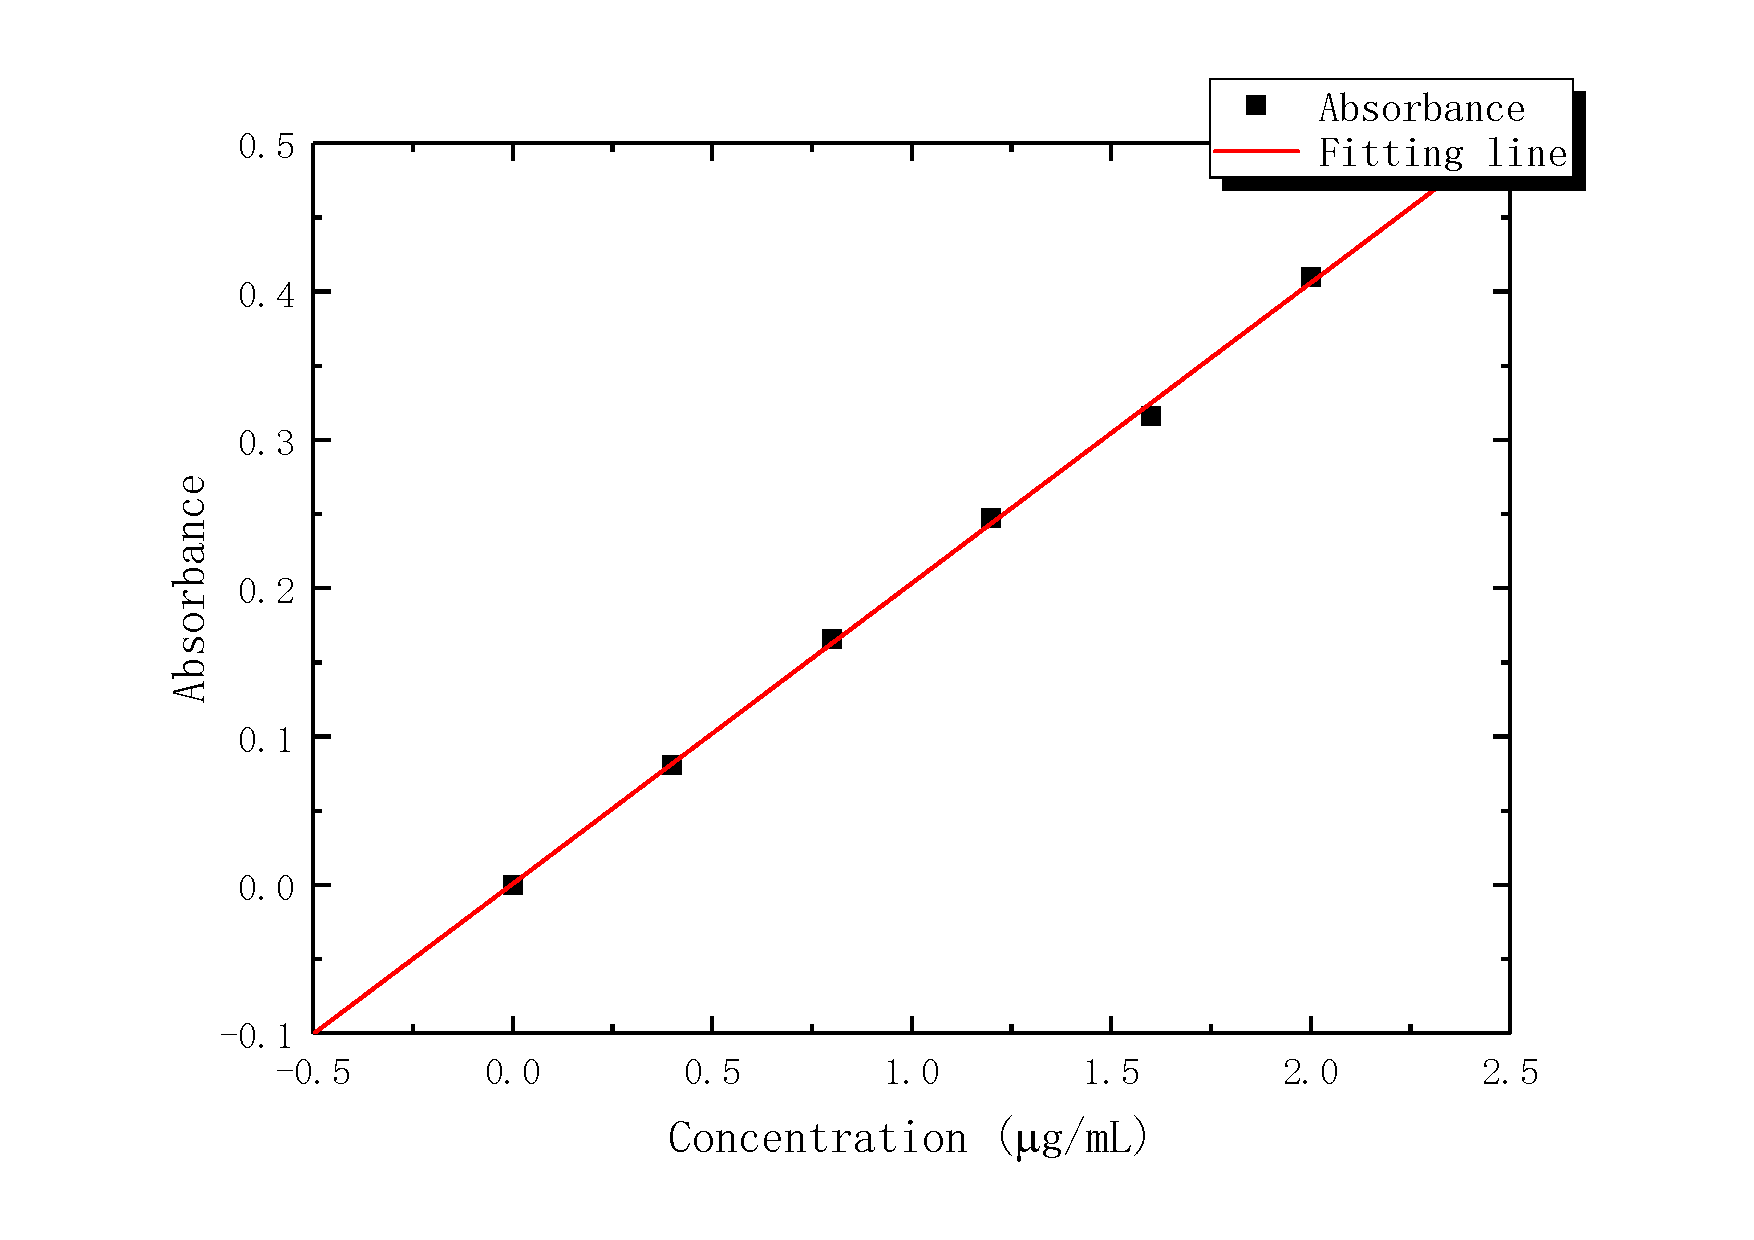
\includegraphics[width=\linewidth]{Fig1.pdf}
    \caption{standard curve}
    \label{fig1}
\end{figure}

\paragraph{Composition determination}

\subparagraph{By molar ratio method}

 The function of fitting line on the left is $y=0.742x+0.0264(R=0.9979)$, and the function of fitting line on the right line is $y=0.254(R=1)$ which are shown below in Figure~\ref{fig2}. According to the figure, we know coordination number measured by molar ratio method is 3.07.

\begin{table}[H]
    \caption{Molar ratio method}
    \label{tab.Mrm}
    \begin{tabular}{lcccccccc}
    \toprule
    Index         &  1  &  2  &  3  &  4  &  5  &  6  &  7  &  8  \\
    \midrule
    $V_{phen}/mL$ &1.00 &1.50 &2.00 &2.50 &3.00 &3.50 &4.00 &4.50 \\
    $V_{Fe}/mL$   &1.00 &1.00 &1.00 &1.00 &1.00 &1.00 &1.00 &1.00 \\
    $\frac{V_{phen}}{V_{Fe}}$
                  &1.00 &1.50 &2.00 &2.50 &3.00 &3.50 &4.00 &4.50 \\
    Absorbance    &0.100&0.140&0.172&0.213&0.252&0.254&0.254&0.254\\
    \bottomrule
    \end{tabular}
\end{table}

\begin{figure}[H]
    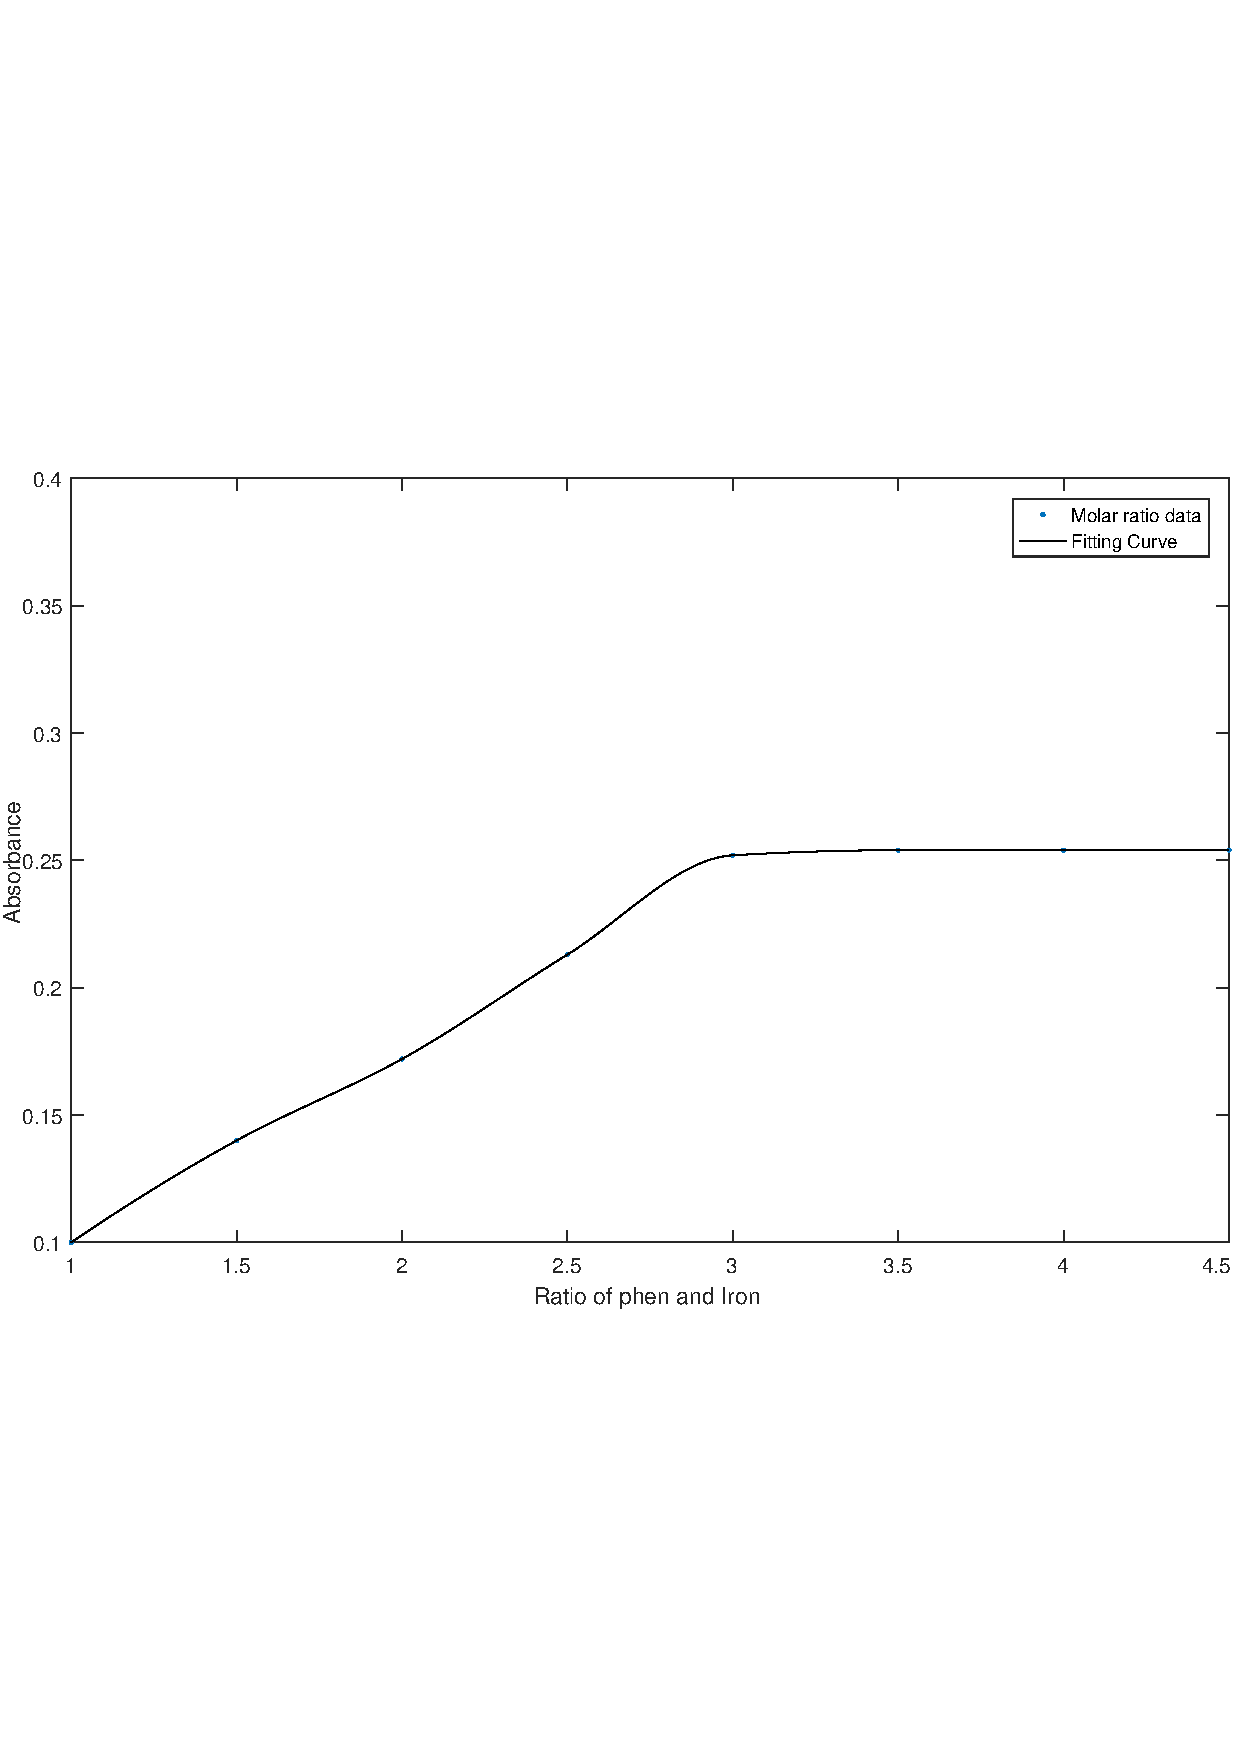
\includegraphics[width=\linewidth]{Fig2.pdf}
    \caption{Molar ratio method}
    \label{fig2}
\end{figure}

To some extent, the correlation coefficient reflects the superiority of the molar ratio method in the terms of accuracy. A reason why it is more accurate than Job method is that when $\frac{V_{phen}}{V_{Fe}}\geq3$, the slope of the line is almost 0 in theory. So compared with Job method, the molar ratio method’s correlation coefficient is closer to 1 which indicates better precision. In a word, as for studying more general coordination compound, typically whose coordination number is not 1, the molar ratio method behaves much better. According to the figure, we know coordination number measured by Job method is 2.79.

\subparagraph{By Job method}

We use $T_L$ to represent $\frac{V_{phen}}{V_{Fe}+V_{phen}}$. When $T_L<0.75$, the fitting line is $y=0.7079x-0.02057(R=0.9966)$, and when $T_L\geq3.0$, the fitting line is $y=-1.874x+1.881(R=0.9363)$ which are shown below in Figure~\ref{fig3}.

\begin{table}[H]
    \caption{Job method}
    \label{tab.Jbm}
    \begin{tabular}{lcccccccccccc}
    \toprule
    Index
    & 1 & 2 & 3 & 4 & 5 & 6 & 7 & 8 & 9 & 10& 11& 12\\
    \midrule
    $V_{phen}/mL$
    &0.0&1.8&3.0&4.0&4.8&5.3&5.7&6.0&6.2&6.4&6.6&8.0\\
    $V_{Fe}/mL$
    &8.0&6.2&5.0&4.0&3.2&2.7&2.3&2.0&1.8&1.6&1.4&0.0\\
    $T_L$
    &   &0.23&0.38&0.50&0.60&0.67&0.71&0.75&0.78&0.80&0.83& \\
    Absorbance
    &   &0.141&0.252&0.330&0.410&0.441&0.490&0.490&0.405&0.368&0.340& \\
    \bottomrule
    \end{tabular}
\end{table}

\begin{figure}[H]
    \includegraphics[width=\linewidth]{Fig3.pdf}
    \caption{Job method}
    \label{fig3}
\end{figure}

The reason why the measured coordination number is smaller than theoretical number is when $T_L\geq3.0$, we only use four points to fit the line, and less points means less accuracy, which is unavoidable when the coordination number isn't 1. Besides, the slope of the theoretical line on the right is so great, which indicates a large relative deviation.

\paragraph{Purity measurement of \ce{FeC2O4}$\cdot$2\ce{H2O}}

\subparagraph{By standard curve}
We apply the standard curve to determine the concentration of iron in our self-made \ce{FeC2O4}$\cdot$2\ce{H2O} sample, therefore getting purity easily by simply calculating: \[\omega=\frac{c_{Fe}\times250mL\times179.9 g/mol}{m_{sample}}\].

\begin{table}[H]
    \caption{Purity Measurement by standard curve}
    \label{tab.Pcurve}
    \begin{tabular}{lcccc}
    \toprule
    Possesor      &Mass/g & Absorbance &$c_{Fe}/\mu g\cdot mL^{-1}$& purity   \\
    \midrule
    Xiao Tan      &0.2083 & 0.546      & 2.52   &$97.2\%$  \\
    Jia-Ye Luo    &0.2170 & 0.534      & 2.46   &$91.1\%$  \\
    Xin-Yang Zhao &0.2023 & 0.501      & 2.31   &$91.8\%$  \\
    Cong Wen      &0.2020 & 0.509      & 2.35   &$93.5\%$  \\
    Xiao-Jie Zhou &0.2048 & 0.517      & 2.38   &$93.4\%$  \\
    Zi-Han Zhao   &0.2184 & 0.530      & 2.44   &$89.8\%$  \\
    \bottomrule
    \end{tabular}
\end{table}

\subparagraph{By titration method}
We can first get the concentration of standard potassium permanganate solution easily using data from Table~\ref{tab.CalMn} by calculating: \[c_{\ce{KMnO4}}=\frac{2}{5}\times\frac{m_{\ce{NaC2O4}}}{134.0 g/mol\times V_{0average}}=0.01895mol/L\].

\begin{table}[H]
    \caption{standard of \ce{KMnO4}}
    \label{tab.CalMn}
    \begin{tabular}{ccc}
    \toprule
    Index\textsuperscript{\emph{a}}&$V_0/mL$&$V_{0average}/mL$\\
    \midrule
    1    & 24.44 &\\
    2    & 24.42 & 24.43\\
    3    & 24.42 &\\
    \bottomrule
    \end{tabular}\\
    \textsuperscript{\emph{a}}:Mass of sample \ce{NaC2O4}=6.2013 g
\end{table}

\begin{table}[H]
    \caption{Titration of \ce{FeC2O4}$\cdot$2\ce{H2O}}
    \label{tab.Tit}
    \begin{tabular}{ccccccc}
    \toprule
    Index\textsuperscript{\emph{a}}&$V_{1start}/mL$&$V_{1end}/mL$&$V_{1average}/mL$&$V_{2start}/mL$& $V_{2end}/mL$&$V_{2average}/mL$\\
    \midrule
    1    & 0.10 & 30.60 &       & 0.00 & 9.85 &     \\
    2    & 0.00 & 30.48 & 30.49 & 0.00 & 9.90 & 9.85\\
    3    & 0.00 & 30.50 &       & 0 00 & 9.80 &     \\
    \bottomrule
    \end{tabular}\\
    \textsuperscript{\emph{a}}:Mass of sample \ce{FeC2O4}$\cdot$2\ce{H2O} =1.8012 g;
\end{table}

Then we can easily calculate the purity by calculating: \[\omega=\frac{5}{2}\times\frac{V_{2average}\times c_{\ce{KMnO4}}\times179.9 g/mol}{m_{sample}}\times\frac{250mL}{25mL}=93.2\%\]

And the comparision of purity measured betweem titration method and spectrophotometry is shown in Table~\ref{tab.Res}.

\begin{table}[H]
    \caption{Purity comparision}
    \label{tab.Res}
    \begin{tabular}{ccc}
    \toprule
           & Titration & standard\\
    \midrule
    Purity & $93.2\%$  & $93.4\%$   \\
    \bottomrule
    \end{tabular}
\end{table}

We find the result of using standard curve is congrent with that of using titration method, therefore validating the accuracy of spectrophotometry.

% ██████  ██████  ███    ██  ██████ ██      ██    ██
%██      ██    ██ ████   ██ ██      ██      ██    ██
%██      ██    ██ ██ ██  ██ ██      ██      ██    ██
%██      ██    ██ ██  ██ ██ ██      ██      ██    ██
% ██████  ██████  ██   ████  ██████ ███████  ██████


\section{Conclusion}
We report that using spectrophotometry to determine iron of micro even trace quantity is effective and meets the requirements of green chemistry. And we apply orthogonal experimental design to optimize the combination of some factors. Meanwhile, we knew the ratio of phen and iron in the complex is 3:1 and drew to a conclusion that molar ratio method is more general and effective in determine composition of coordinary compound. Then we plotted a standard curve, with which we can predict the concentration of iron in unknown sample. The result is very accurate, which is validated by measuring the purity of \ce{FeC2O4}$\cdot$2\ce{H2O}. Most importantly, the chromoginice agent can be specifically chosen in various conditions so spectrophotometry can be widely applied to diverse ions of diverse quantity.



\begin{acknowledgement}

The authors thank Dr.Hong-Jin Chen and Dr.Jian-Tao Zai for their imparting traditional as well as up-to-date knowledge to us and correct guidance in our experiment. The authors also thank the assistant teacher Kai He for his meticulous care and helping us to master experimental operation.

\end{acknowledgement}

\bibliography{SDIUP}

\end{document}
